General structure and tasks of an early detection system were already described in chapter \ref{early_detection_system}.
As it was mentioned before, an early detection system consists of two different components:

\begin{enumerate} 
    \item Several small embedded devices, deployed in the field. They capture images with thermal camera, process them and send results over wireless network.
    \item One gateway, which is receiving results, and relays them to an application server over internet connection.
\end{enumerate} 

In this chapter we focus on the structure and design of deployed embedded system,both from hardware and firmware point of perspective.
We also describe construction of an application server, how received data is processed, stored and presented.

The general block diagram of an embedded system with a thermal camera is presented on the Figure \ref{system_diagram} 

\begin{figure}[ht]
        \centering
        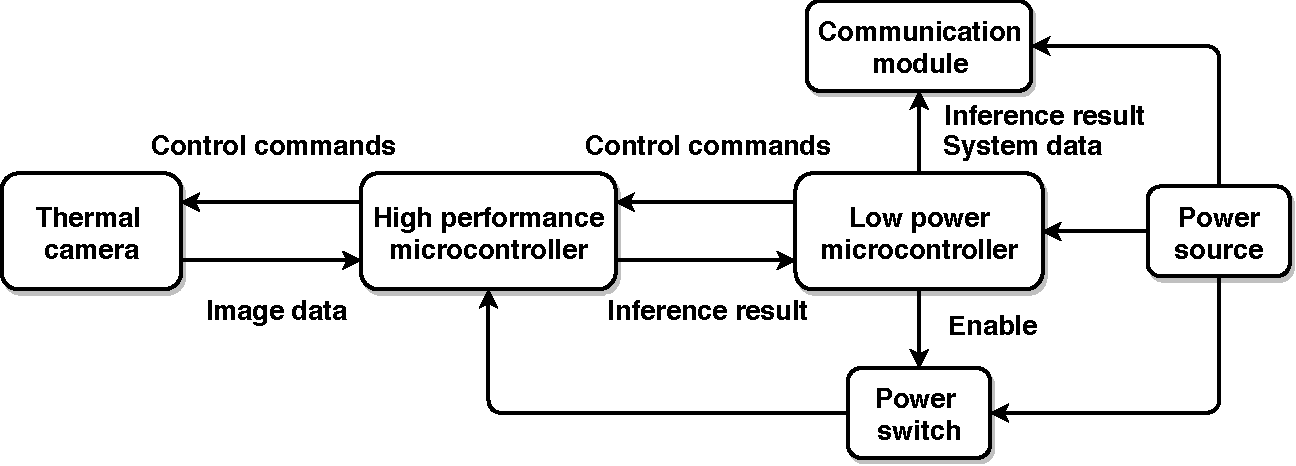
\includegraphics[width=1.0\linewidth]{system_diagram.pdf} 
        \caption{ General block diagram of an embedded system}
        \label{system_diagram}
\end{figure}

Embedded system will consist of two different microcontrollers with two distinct tasks, a thermal camera, PIR sensor, wireless communication module, power switch and battery.

Powerful, high performance microcontroller and thermal camera are turned off, to conserve battery life.
A less capable, but low power microcontroller will spend most the time in sleep, waiting for a trigger from PIR sensor.
PIR sensor will point in the same direction as the thermal camera and will detect any IR radiation of a passing object.

If an object passes PIR's field of vision, it triggers it, which in consequently wakes up a low power microcontroller.
Microcontroller will then enable power supply to high performance microcontroller and thermal camera, and send a command request for image capture and processing.

Thermal camera only communicates with high performance microcontroller, which configures it and requests image data.
That data is then inputted into neural network algorithm and an probability results are then returned to a low power microcontroller.
low power microcontroller then packs the data and sends it over radio through wireless communication module.
Power source to high performance microcontroller and thermal camera is then turned of to conserve power.
Diagram of described procedure can also be seen on Figure \ref{system_flow}.

\begin{figure}[ht]
        \centering
        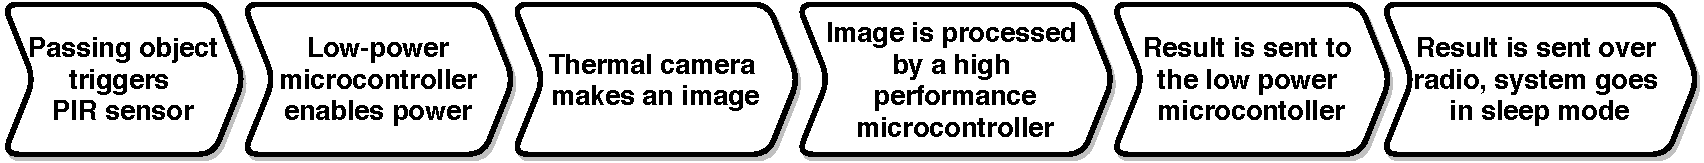
\includegraphics[width=1.0\linewidth]{system_flow.pdf} 
        \caption{ Diagram describing behavior of embedded early detection system} 
        \label{system_flow}
\end{figure}


\section{ Hardware}

In this section we present concrete components that we used to implement the embedded part of the early detection system.
Hardware version of embedded system diagram is presented on the Figure \ref{hardware_diagram}.
It should be noted that we did not include specific power source into the diagram.
Wisent Edge tracker board is general enough to work with different power sources, such as non-chargeable or chargeable batteries and or solar cells.

\begin{figure}[ht]
        \centering
        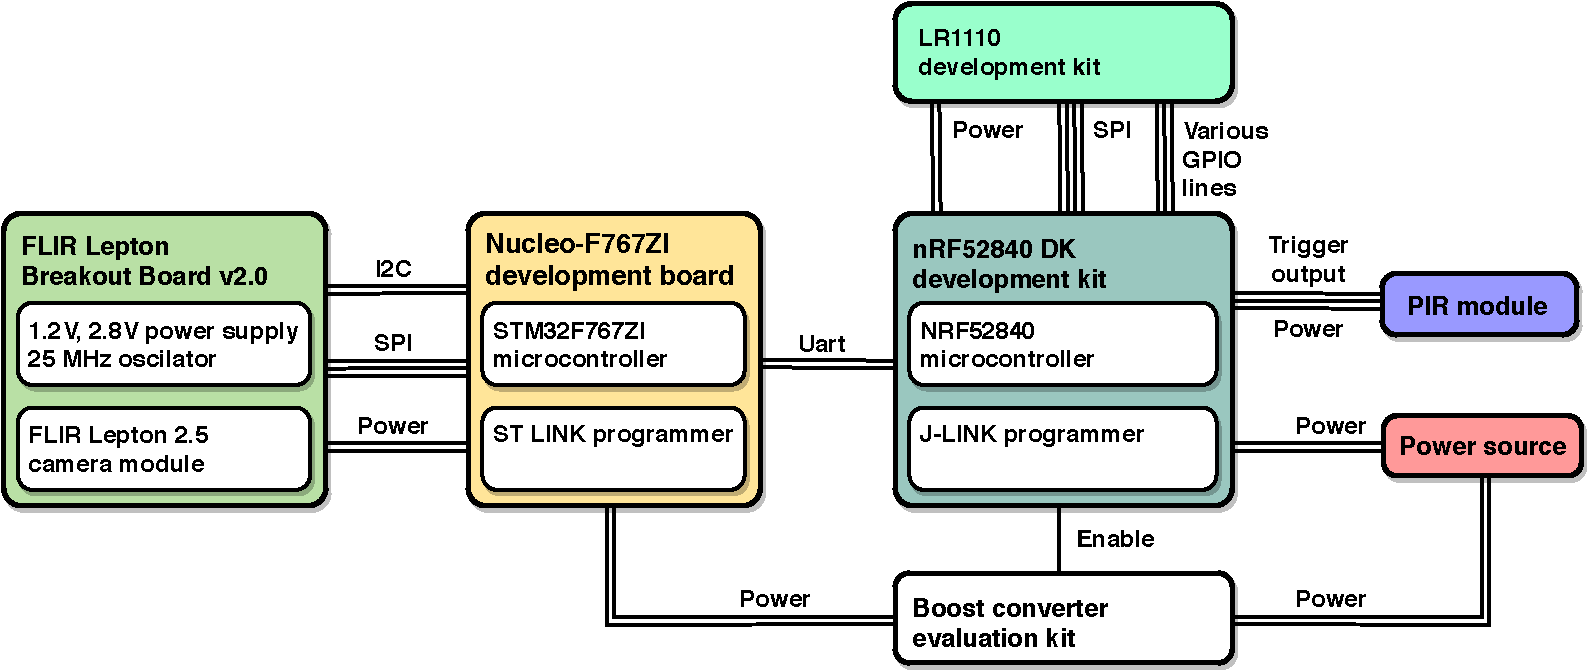
\includegraphics[width=1.0\linewidth]{hardware_diagram.pdf} 
        \caption{ Hardware diagram of embedded early detection system} 
        \label{hardware_diagram}
\end{figure}

\subsection{ Nucleo-F767ZI}

Nucleo-F767ZI (seen on Figure \ref{nucleo}) is a development board made by STMicroelectronics.
Board features STM32F767ZI microcontroller with Cortex-M7 core, which has 2 \si{\mega\byte} of flash, 512 \si{\kilo\byte} of SRAM and can operate at clock speed of 216 \si{\mega\hertz}.
It also features different memory caches and flash accelerator, which provide extra boost in performance.
It is convenient to program it, as it includes on board ST-LINK programmer circuit.

We chose this microcontroller simply because it is one of more powerful general purpose microcontrollers on the market.
As we knew that neural networks are computationally expensive to compute and that models can be quite large in terms of memory, we selected it knowing that we can always scale down, if we have to.

\begin{figure}[ht]
        \centering
        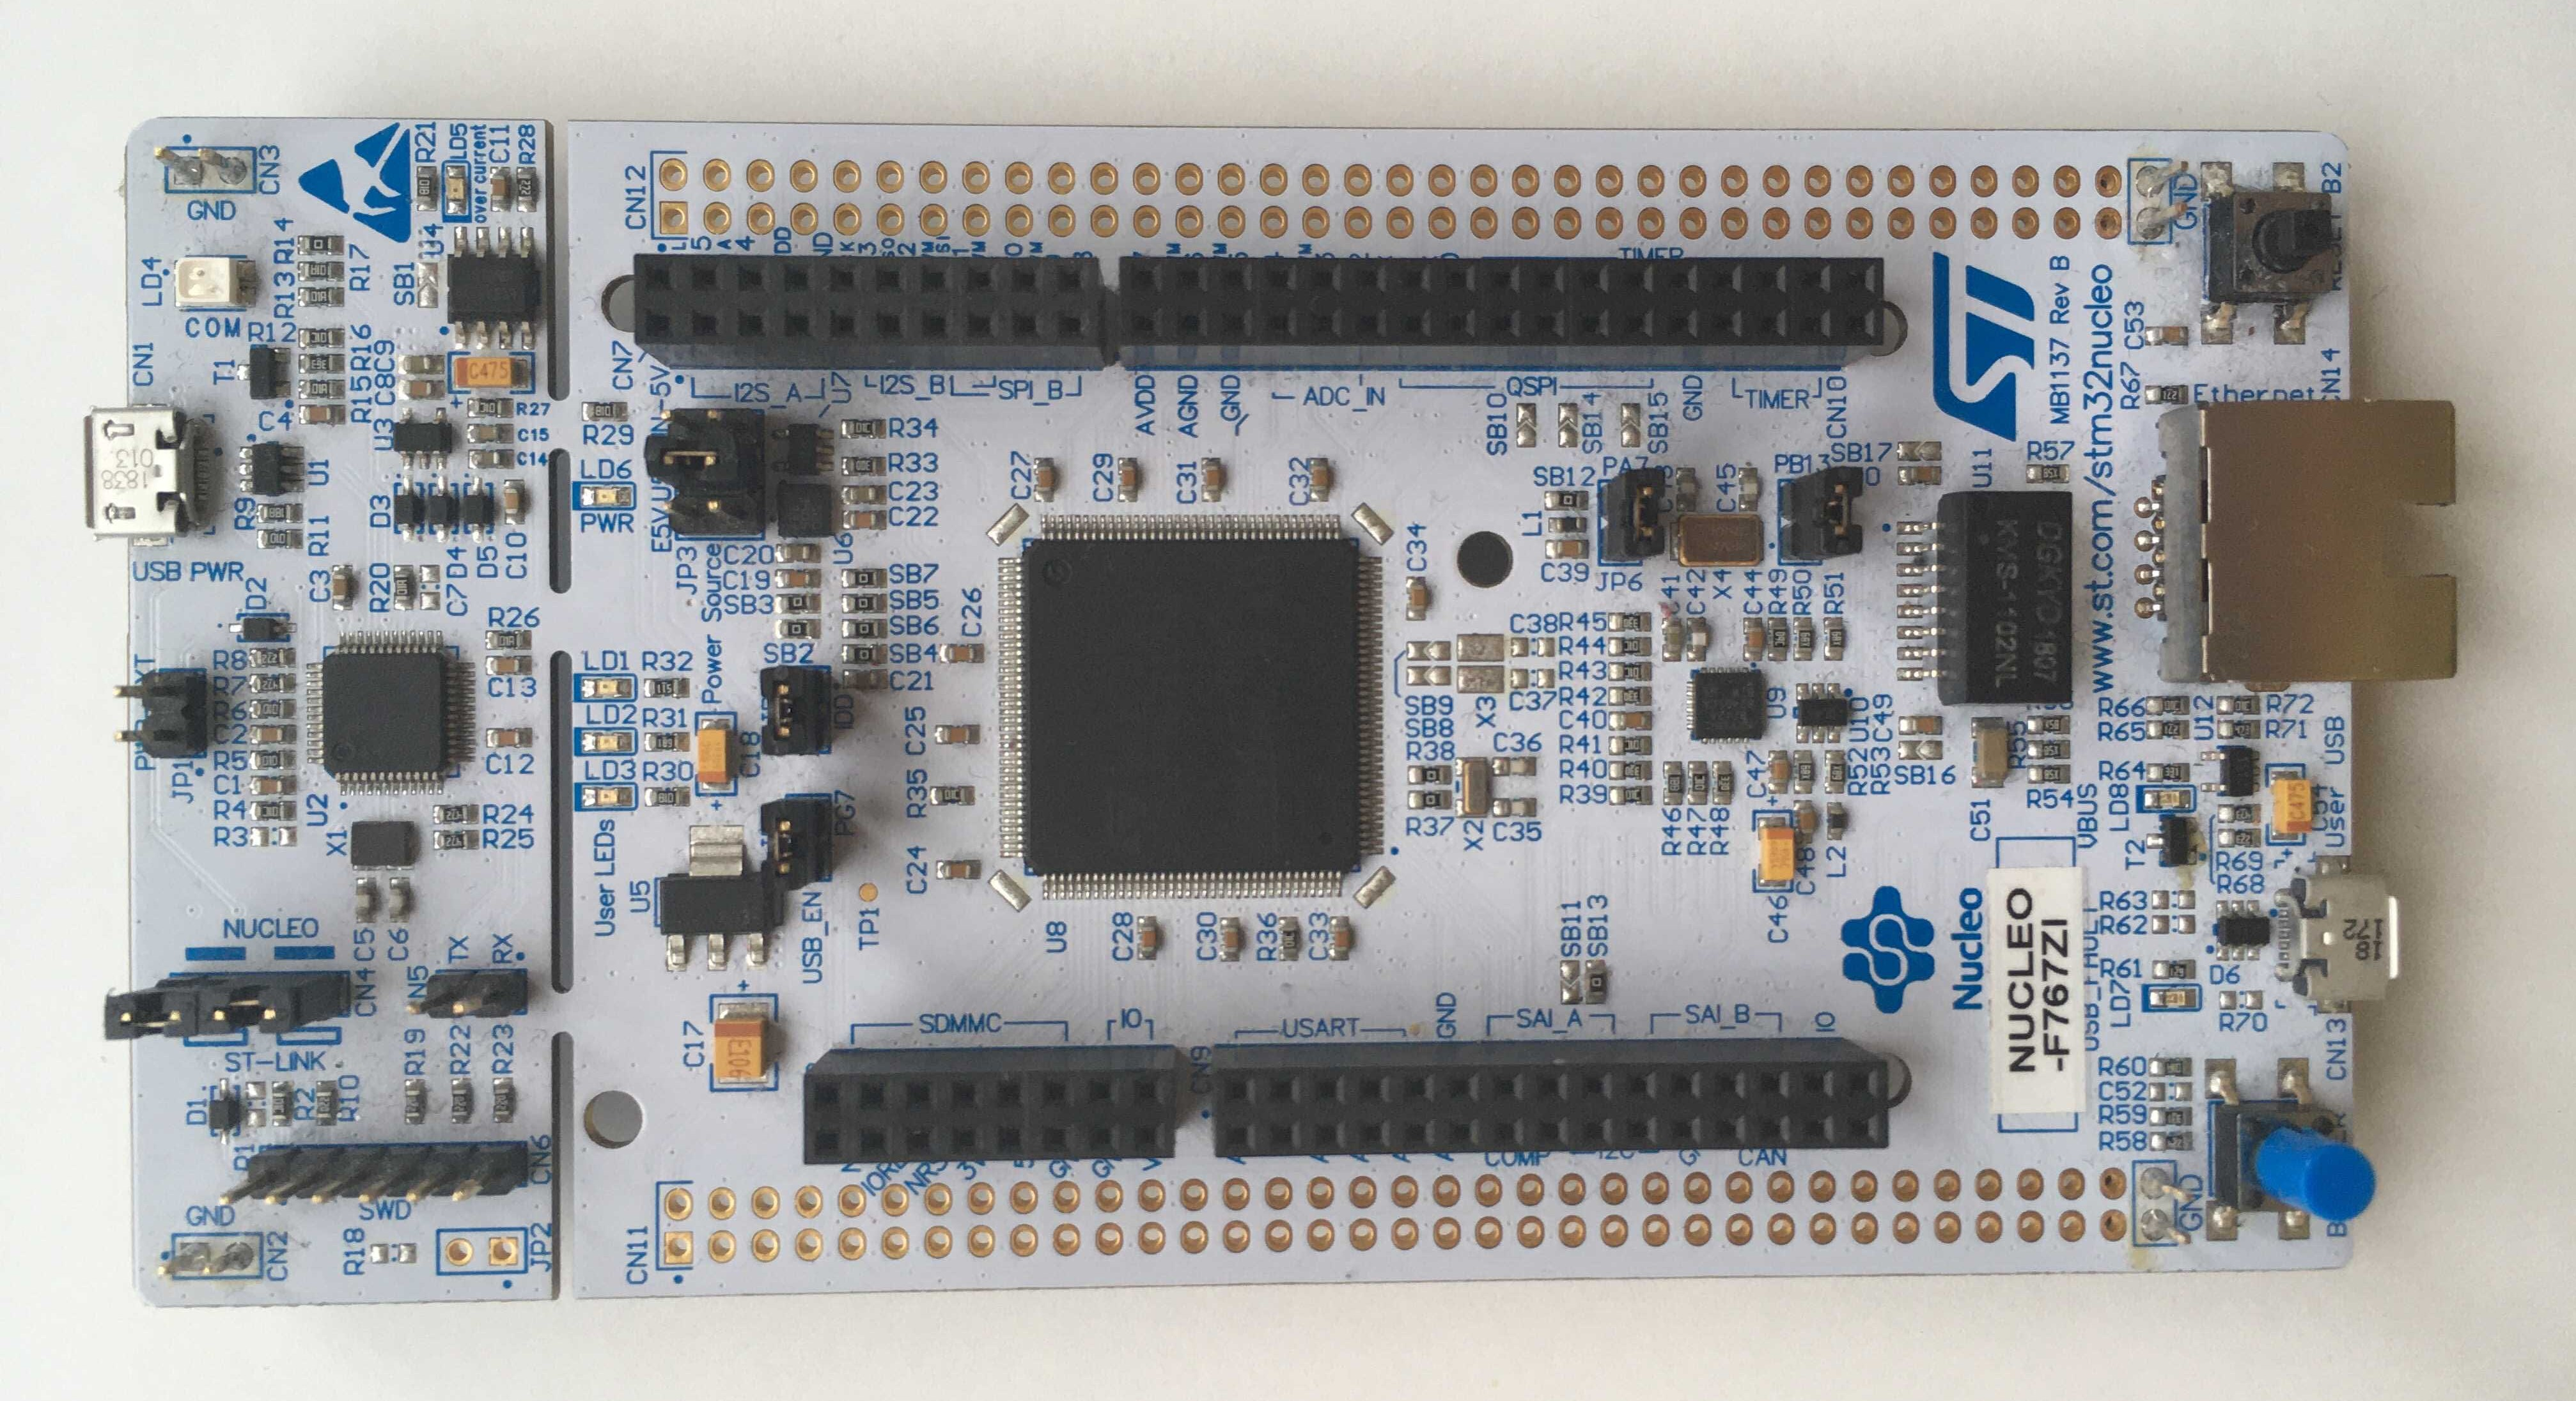
\includegraphics[height= 8cm]{nucleo.jpg} 
        \caption{ Nucleo-F767ZI development board} 
        \label{nucleo}
\end{figure}


\subsection{ Wisent Edge tracker}

For the part of the system which had to contain low power microcontroller, communication module and power control for Nucleo-F767ZI board we decided to use Wisent Edge tracker board.
Wisent Edge (seen on Figure TODO ADD IMAGE) is a tracker solution, specifically developed for conserving endangered wildlife animals.
It is one of many tracker solutions that were a product of open-source\footnotemark collaboration between Irnas and company Smart Parks, which provides modern solutions in anti-poaching and animal conservation areas.

\footnotetext{ As a part of OpenCollar project, the design of Wisent Edge is open-source and available on GitHub\cite{opencollar}, alongside other hardware and firmware tracker projects.}

The main logic on the board is provided by Nordic Semiconductor's NRF52840 microcontroller with Cortex-M4 core, which has 1 \si{\mega\byte} of flash, 256 \si{\kilo\byte} of RAM and Bluetooth 5 support.
NRF52840 has consumption of 0.5 \si{\micro\ampere} in sleep mode, which makes it ideal for our purpose.

Wisent Edge also features Semtech's LR1110 chip (which acts as a LoRa transceiver, GNSS and WiFi location module) and another GPS module, U-blox's ZOE-M8G\footnotemark.
There is a ceramic GPS antenna on board and a U.FL connector to which a dual band Wifi, Bluetooth and LoRa antenna can be attached.

\footnotetext{Reason for two GNSS modules is that although LR1110 chip can provide extremely power efficient location information, it's accuracy is smaller when compared to ZOE-M8G and it can only be resolved after sending it to an application server\cite{irnas_lr1110}.}

As geopositioning of system was not primary concern, GNSS functionalities were not used, however they might be usefull in future.

Power control of a Nucleo-F767ZI board and FLIR camera is provided by a dual channel p and n MOSFET, circuit can be seen on Figure \ref{mosfet}.
Circuit functions as a high side switch, with microcontroller pin driving enable line.
When enable line is low, n MOSFET is closed, therefore p MOSFET is also closed, as it is pulled high by resistor R1.
When enable line is high, n MOSFET is opened, therefore gate of p MOSFET is grounded, which opens the MOSFET.

\begin{figure}[ht]
        \centering
        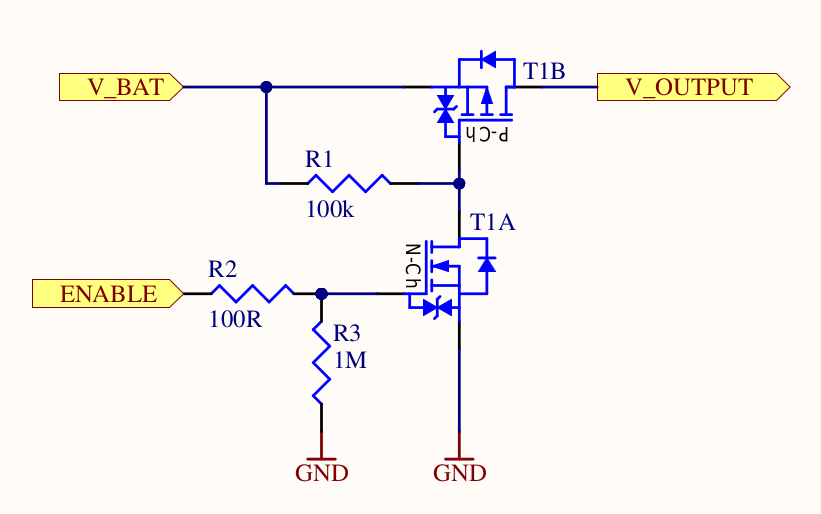
\includegraphics[width=1.0\linewidth]{mosfet.png} 
        \caption{ Dual P and N MOSFET configuration for power switching}
        \label{mosfet}
\end{figure}

\subsection{ Flir Lepton 2.5 camera module and Lepton breakout board}

In section \ref{thermal_cameras} it was described what kinds of thermal cameras exist and how do they work, and in section \ref{choosing_thermal} it was described why FLIR Lepton 2.5 was chosen.
However, not much was said about what sort of support circuitry FLIR camera needs and how do we actually make images with it.

FLIR Lepton camera needs to be powered from two different sources, 1.2 \si{\volt} and 2.8 \si{\volt}, as well it needs a reference clock of 25 \si{\mega\hertz}.
All of this is provided by Lepton breakout board, which can be seen on the Figure \ref{lepton_breakout}.
Front side of the breakout board contains a FLIR module socket and back side has two voltage regulators and a oscillator.
Breakout board can be powered from 3.3 to 5 \si{\volt} and also conveniently breaks out all communication pins in form of headers.

\begin{figure}[ht] 
    \begin{subfigure}[b]{0.5\textwidth}
        \centering
        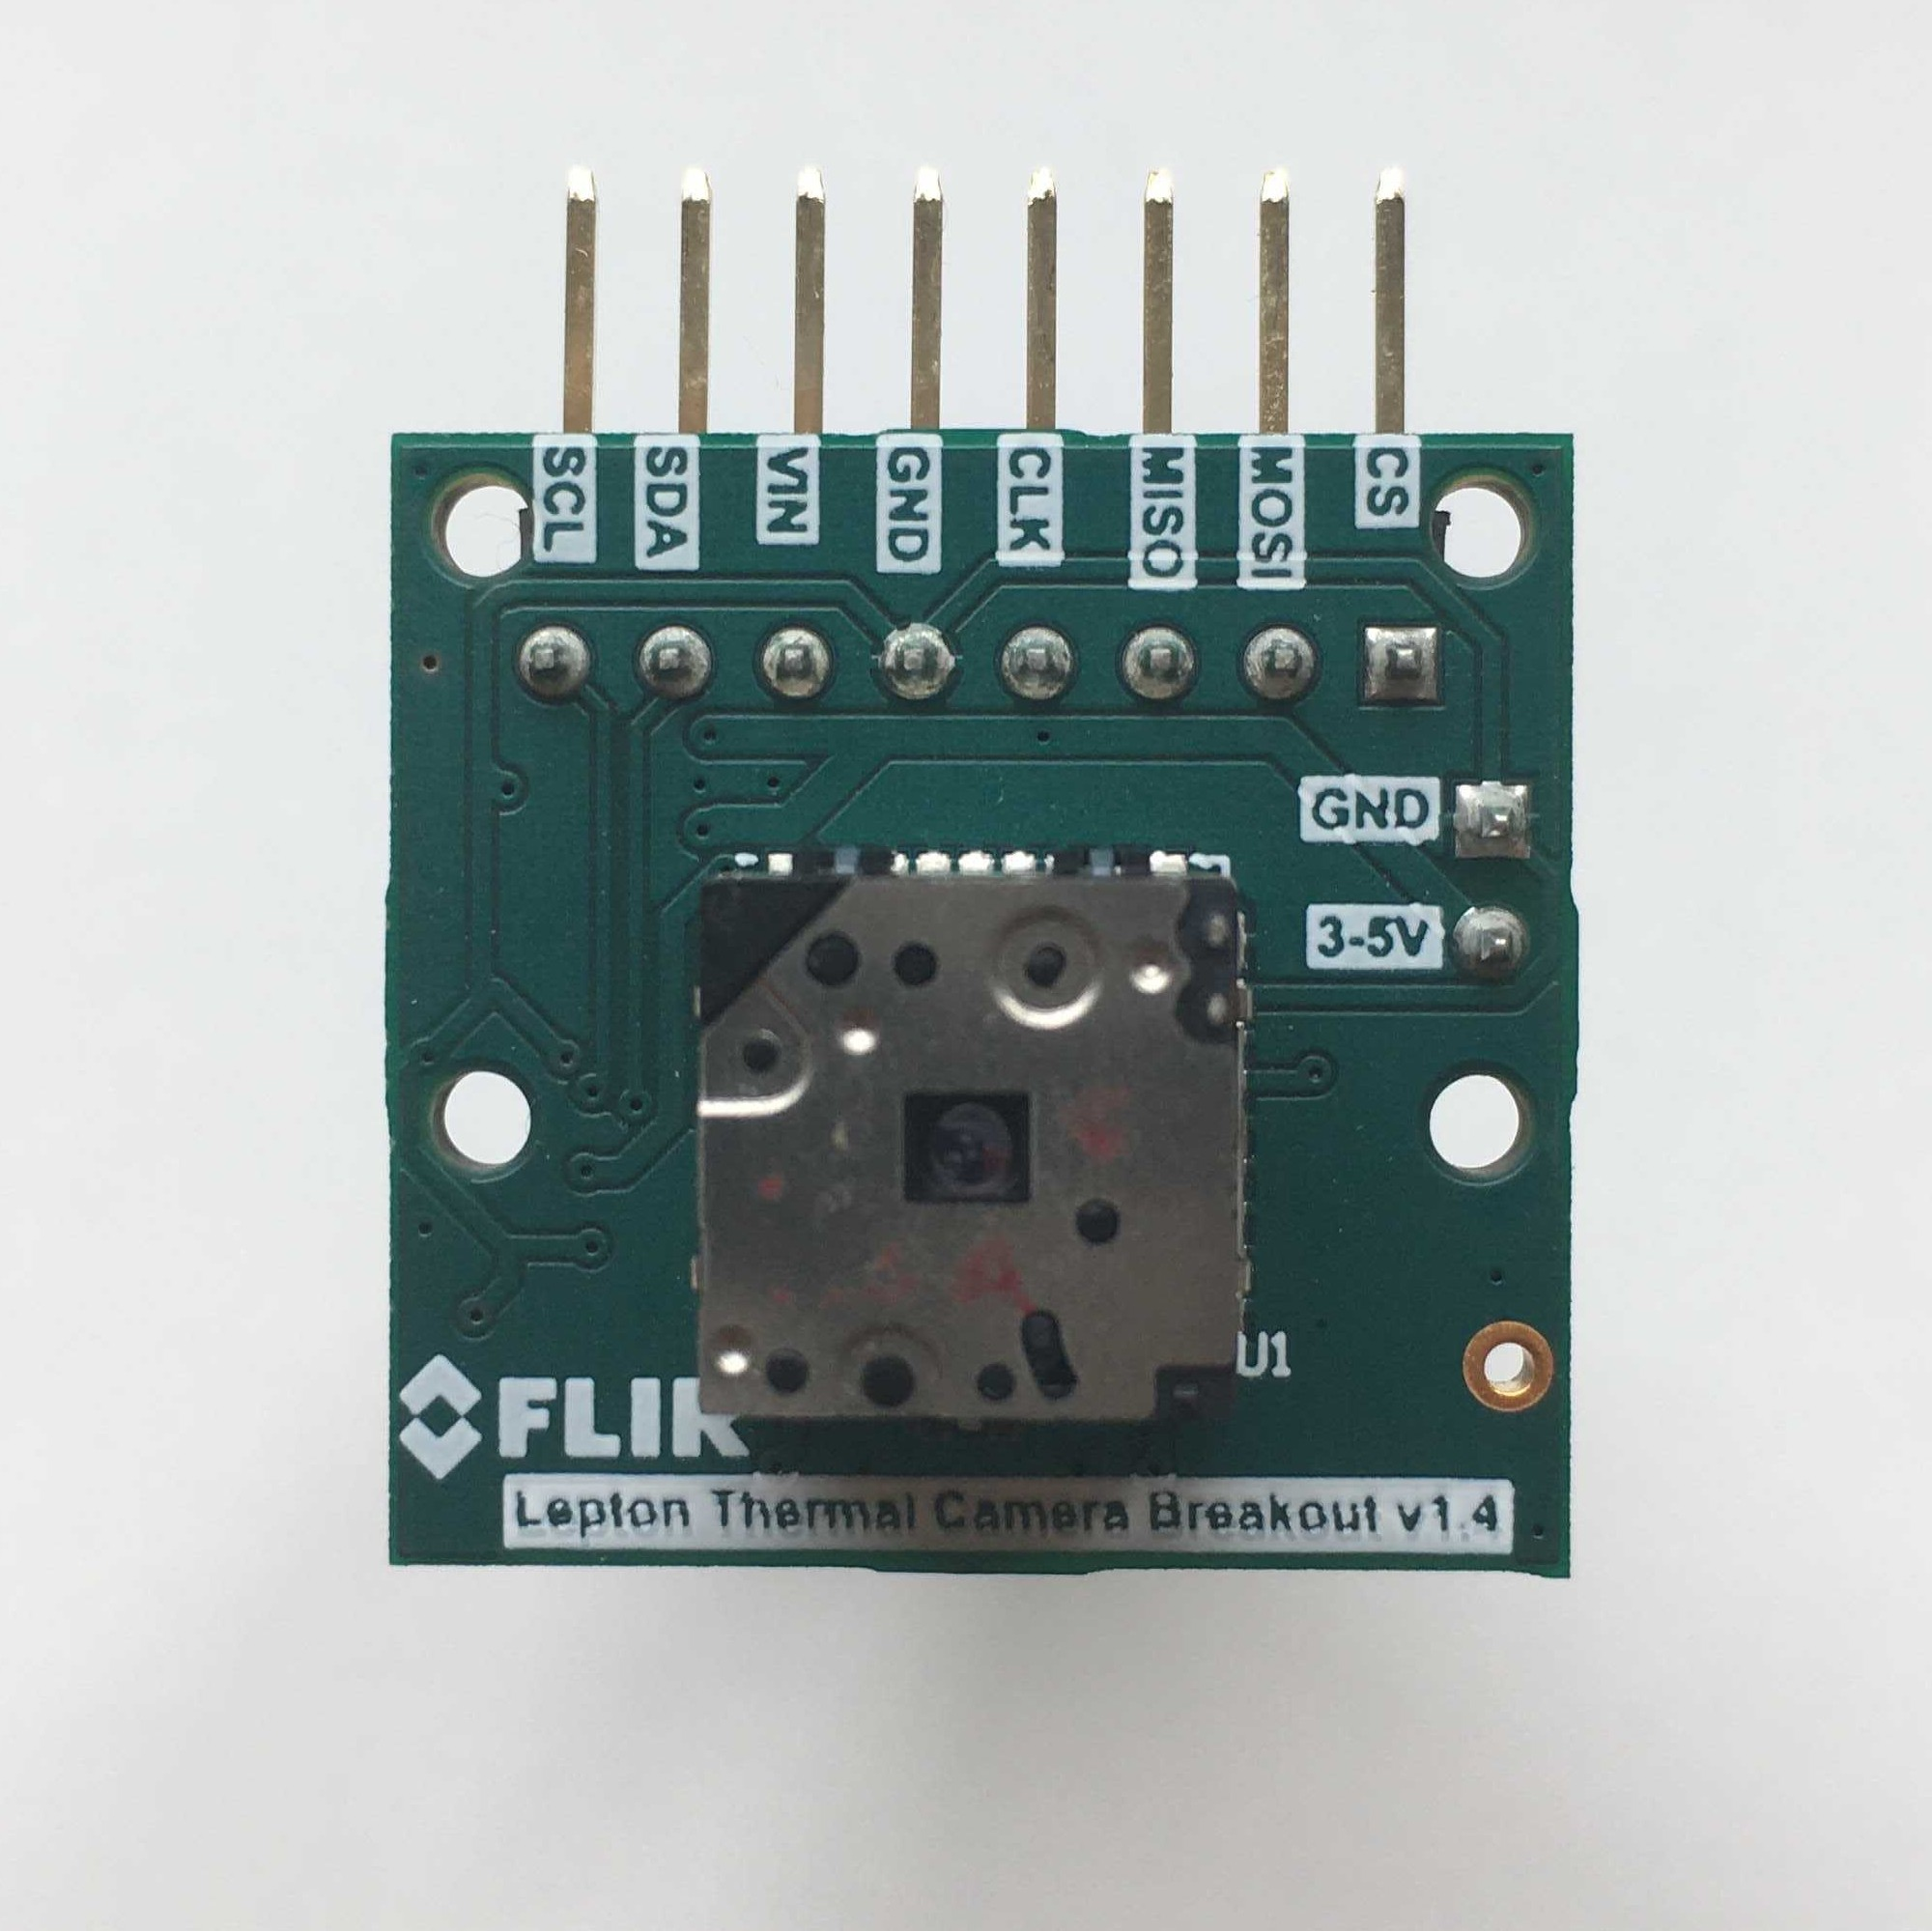
\includegraphics[width=1.0\linewidth]{flir_module_front.jpg} 
    \end{subfigure}
    \begin{subfigure}[b]{0.5\textwidth}
        \centering
        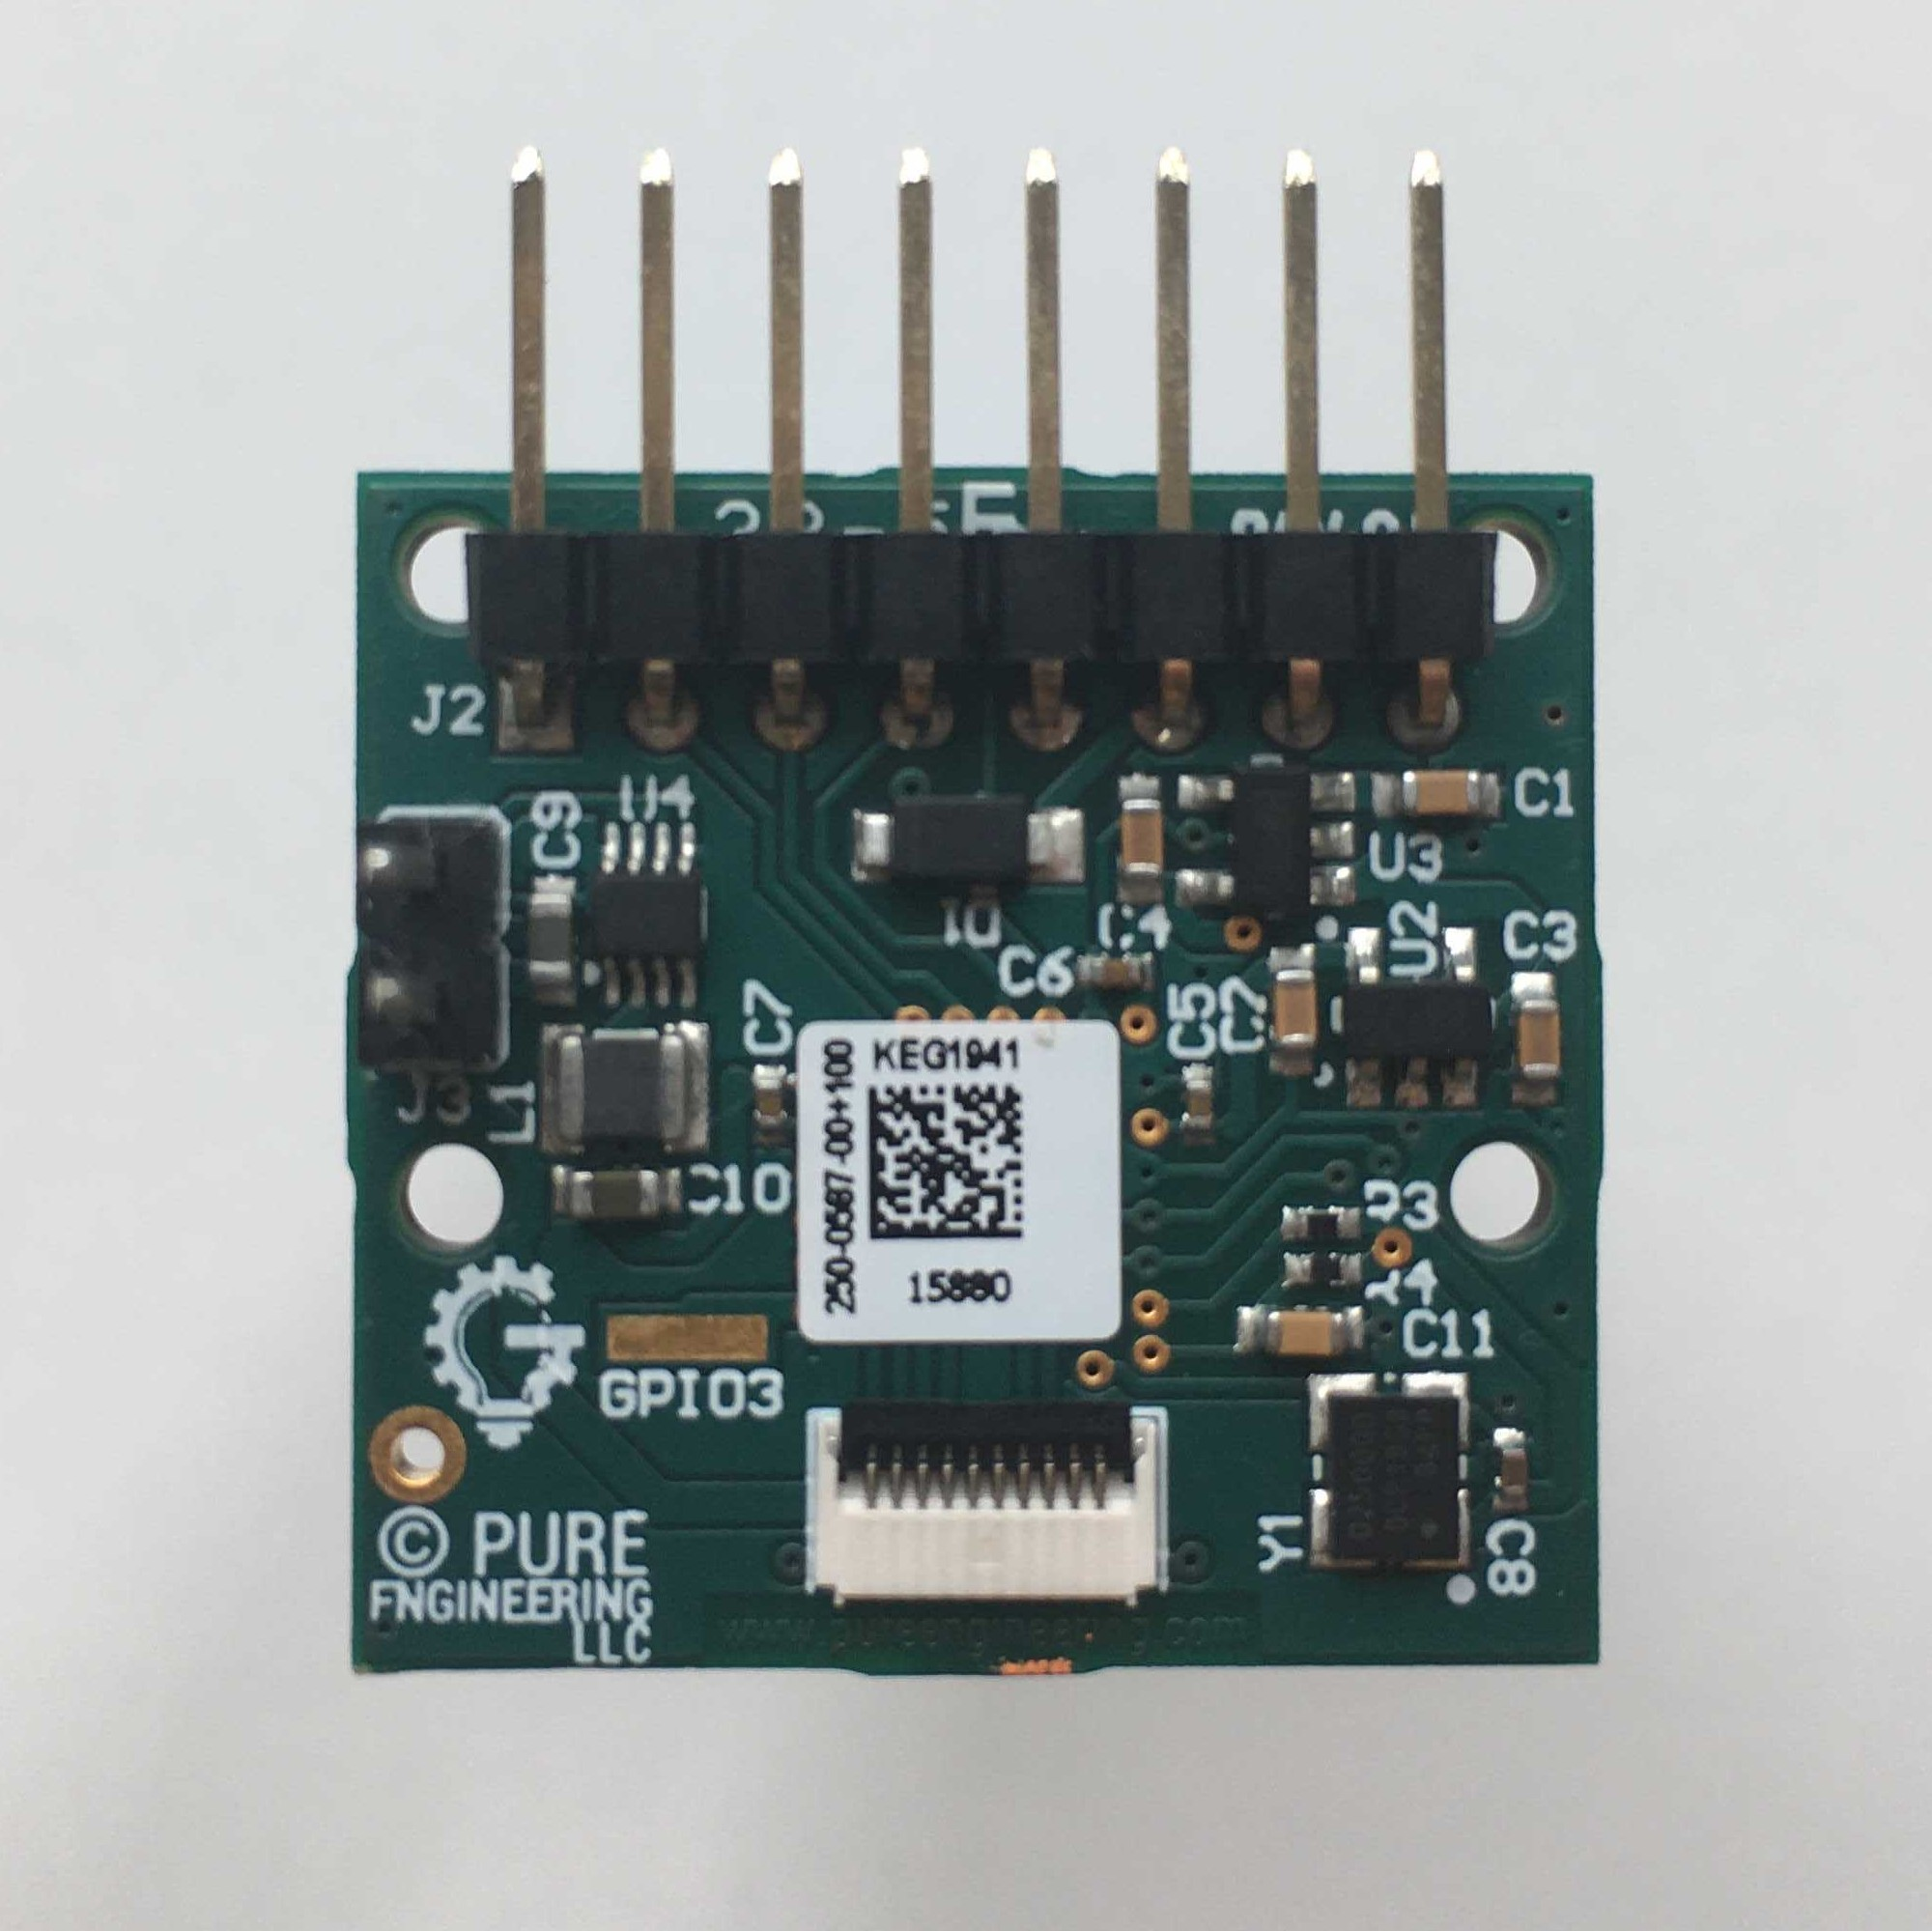
\includegraphics[width=1.0\linewidth]{flir_module_back.jpg} 
    \end{subfigure}
    \caption{ Front and back side of Flir Lepton breakout board with thermal camera module inserted.}
    \label{lepton_breakout}
\end{figure}

FLIR Lepton module itself conatins five different subsystems that work together and can be configured:

\begin{itemize}
    \item AGC – Automatic Gain Control, affects image contrast and quality
    \item SYS – System information
    \item VID – Video processing control
    \item OEM – Camera configuration for OEM customers
    \item RAD – Radiometry
\end{itemize}

AGC subsystem deals with converting a dynamic range of an IR sensor into a compact range that is more suitable for storing and displaying images.
In case of FLIR Lepton this is a 14-bit to 8-bit conversion.
For our purposes AGC subsystem was turned on, as the input to our neural network were 8-bit values.

Microcontroller communicates with FLIR camera over two interfaces: two wire interface (TWI) is used for sending commands and controlling the FLIR camera and Lepton's VoSPI protocol is used for image transfer.

TWI is a variation of an I2C protocol, instead of 8 bits, all transfers are 16 bits.
Internal structure of Lepton's control block can be seen on the Figure \ref{flir_lepton_cci}.
Whenever we are communicating with FLIR camera we have to specify which subsystem are we addressing, what type of action we want to do (get, set or run), length of data and data itself.

\begin{figure}[ht]
        \centering
        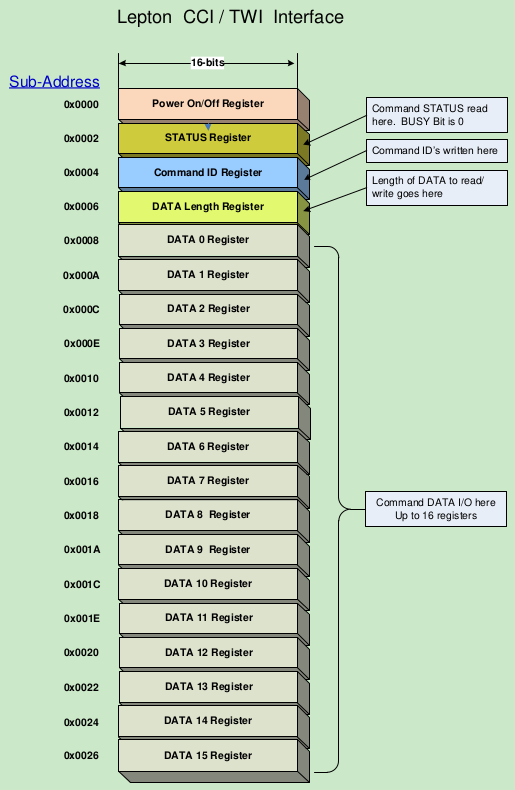
\includegraphics[height=10cm]{flir_lepton_cci.png} 
        \caption{ Command and control interface of FLIR Lepton camera.} 
        \label{flir_lepton_cci}
\end{figure}

Lepton's VoSPI protocol is used only to stream image data from camera module to the microcontroller, which means that MOSI line is not used.
Each image is fits into one VoSPI frame and each frame consists of 60 VoSPI packets.
One VoSPI packet contains an 2 bytes of an ID field, 2 bytes of an CRC field and 160 bytes of data\footnotemark, that represents one image line.

Refresh rate of VoSPI frames is 27 \si{\hertz}, however only every third frame is unique from the last one.
It is a job of the microcontroller to control the SPI clock speed and process each frame fast enough so that next unique frame is not discarded.

\footnotetext{ Because images pixel values fit into 14-bit range by default, it means that one pixel value needs two bytes of data (two most significant bytes are zero). That means that each image line (80 pixels) is stored into 160 bytes. If AGC conversion is turned on, each pixel is then mapped into 8-bit range, however the size of one line in VoSPI packet still remains 160 bytes, 8 most significant bits are simply zeros.}


\subsection{ PIR Sensor}

\section{ Firmware}

\subsection{ Tools and development environment}

For our firmware development we did not chose any of various vendor provided integrated development environments.
We instead used terminal text editor Vim for writing and editing the code.

As we were programming two different microcontrollers, we were using different tools with each one.


\subsubsection{ Development environment for STM32f767ZI}

For building our firmware programs we used GNU Make, build automation that builds software according to user written \textit{Makefiles}.
For compilation we used Arm embedded version of GNU GCC.
To program binaries into our microcontroller we used OpenOCD.

As a hardware abstraction library we used libopencm3, which is a open-source low level library that supports many of Arm's Cortex-M processors cores, which can be found in variety of microcontroller families such as ST's STM32, Toshiba's TX03, Atmel's SAM3U, NXP's LPC1000, Silabs's EFM32 and others.
Libopencm3 provided us with linker files, startup routines, thinly wrapped peripheral drivers and a starting template makefile, which served as a starting point for our project.

As libopencm3 does not provide \verb|printf| functionality out of the box we used excellent library by GitHub user mpaland \cite{printf_lib}


\subsubsection{ Development environment for NRF52840}

To develop firmware for NRF52840 we decided to use The Zephyr OS, which is a small kernel, designed for IoT embedded systems.
Besides usual RTOS functionalities such as tasks, mutexes, semaphores it also provides common driver API for supported microprocessors.

\subsection{ Architecture design}

STM32F767ZI firmware was designed to be very efficient and lean, only truly necessary parts of firmware were implemented.

As seen on Figure \ref{firmware_diagram} we split the firmware into two hardware and application modules.

\begin{figure}[ht]
        \centering
        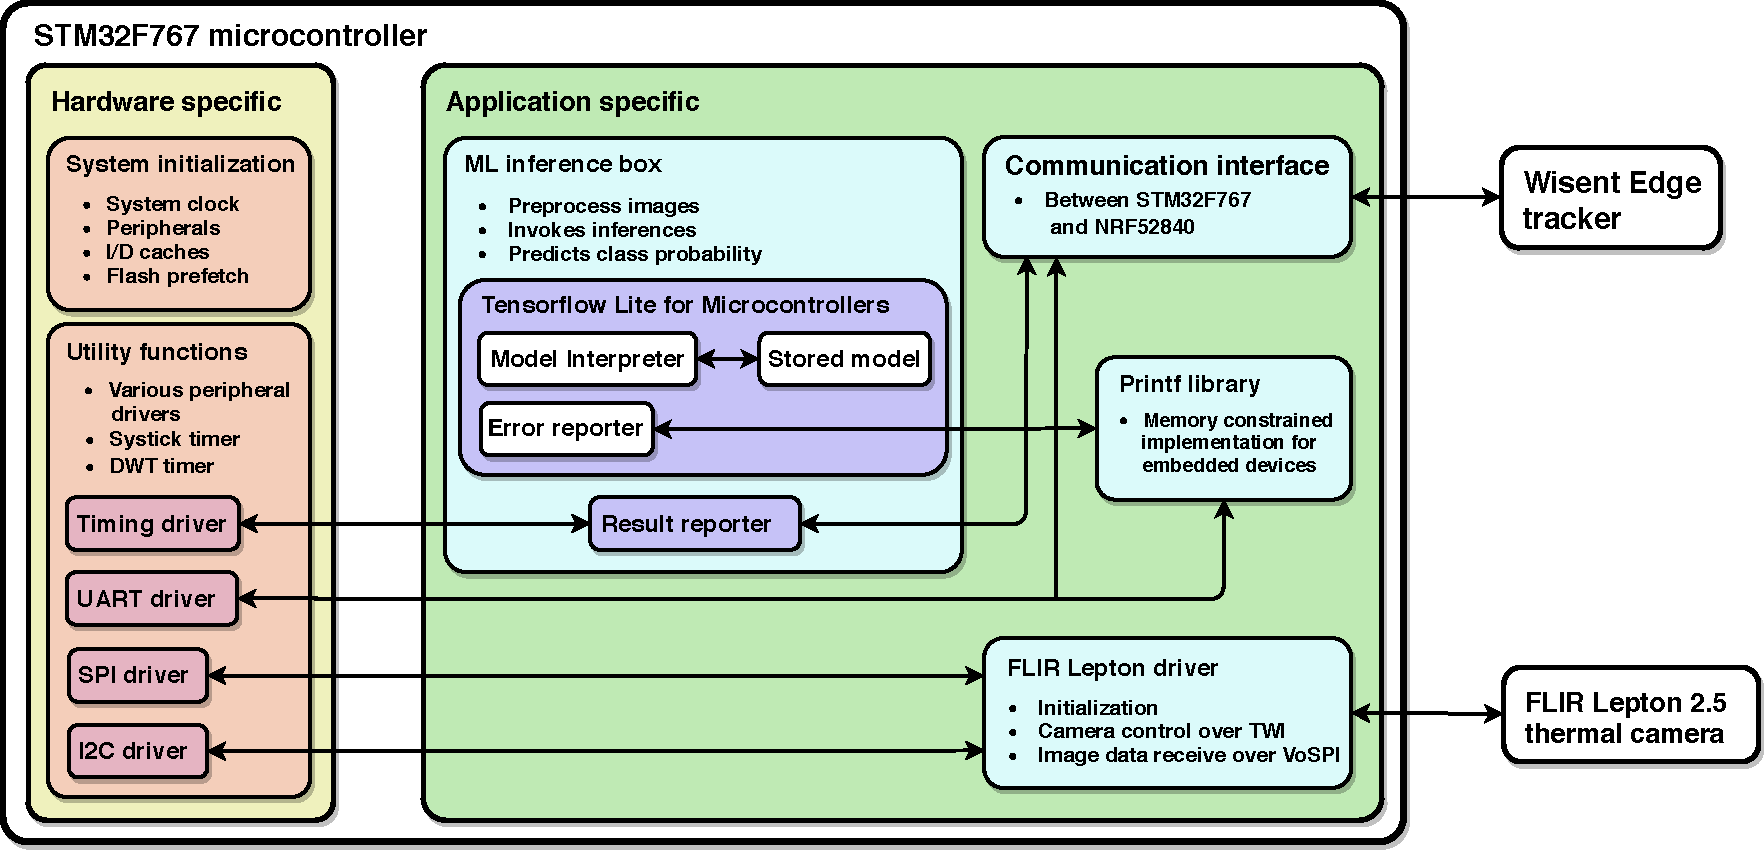
\includegraphics[width=1.0\linewidth]{firmware_diagram.pdf} 
        \caption{ Architecture diagram of the firmware that is running on a STM32F767ZI microcontroller.} 
        \label{firmware_diagram}
\end{figure}

Both modules are lightly coupled, which enables us reuse of the application module on a different hardware sometime in the future.
Hardware specific module is mostly using libopencm3 API to set the system clock and initialize peripherals.
Small function wrappers had to be written to make use of various peripheral drivers more abstract.

FLIR Lepton driver was written from scratch, as many libraries provided either by camera manufacturer or open source communities were too complex and implemented many features which we did not require.

Thanks to TFLite Micro API, ML inference module could be written as a simple black box.
Image data goes in, predictions come out.

TODO describe communication interface between THIS AND WISENT EDGE.


The architecture diagram for NRF52840 can be seen on Figure \ref{firmware_diagram_wisent}.
For NRF52840 microcontroller, we did not had to write any peripheral drivers, as they were provided by Zephyr itself.
Priority was to achieve low power consumption, for which NRF52840 had to spend most of its time in sleep mode, such behavior was easily configurable in Zephyr.

\begin{figure}[ht]
        \centering
        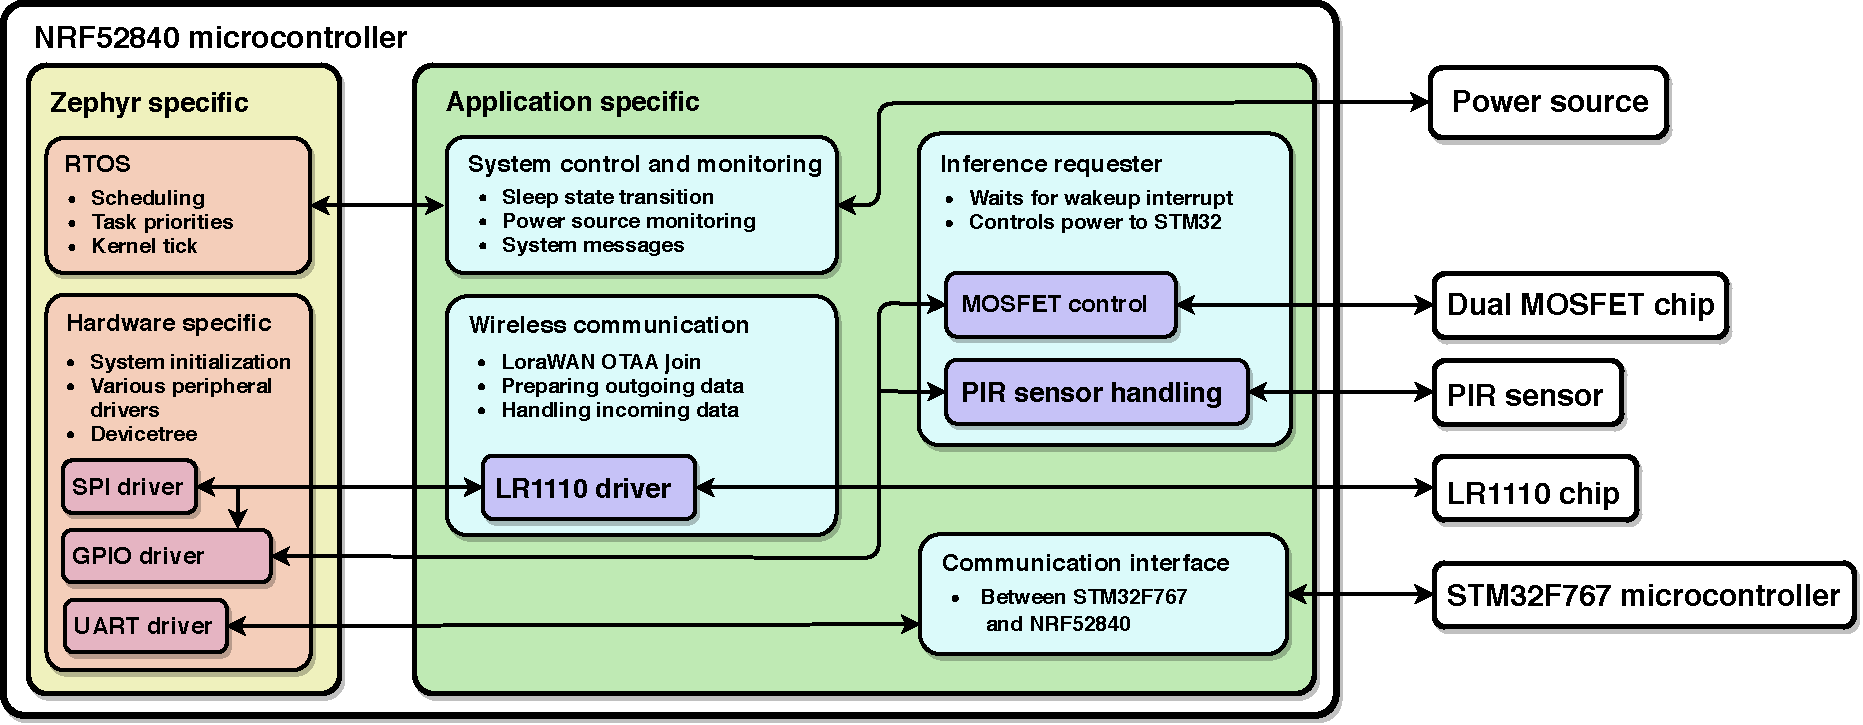
\includegraphics[width=1.0\linewidth]{firmware_diagram_wisent.pdf} 
        \caption{ Architecture diagram of the firmware that is running on a NRF52840 microcontroller.} 
        \label{firmware_diagram_wisent}
\end{figure}

This functionality is encapsulated in inference requester module, which is also waking up the microcontroller when PIR trigger signal is received and controlling the MOSFET.

We also wrote communication module, which takes care of controlling the LR1110 chip, joining LoRaWAN network, preparing outgoing messages and sending them over LoRaWAN network.

TODO describe communication interface between THIS AND WISENT EDGE.


\subsection{ MicroML and build system} \label{build_system_label}

Large part of this thesis was concerned with porting TFLite Micro to libopencm3, our platform of choice.
To understand how this could be done, we first had to analyze how the code is build in TFLite Micro.

To compile source files and build binaries TFLite Micro uses GNU Make.
Main makefile that includes several platform specific makefiles dictates how firmware is built and several scripts which download various dependencies.
By providing command line arguments users decide which example has to be compiled and for which platform.
The build system makes some assumptions about locations of the platform specific files, which in case of example projects are scattered over the whole TensorFlow GitHub repository.

We learned a useful principle while observing the build process. 
Each time we would build an example for a new platform, Make would first compile all TensorFlow files, create a static library out of them, compile specific example source files and then link against library in linking stage.
If we wanted to build firmware for a different example, Make would only had to compile source files of that example and it could reuse previously made library.
As compiling of static library took quite some time, this was an efficient option.

After analyzing the TFLite Micro's build system we created a list of requirements that we wanted to fulfil on our platform.

\begin{enumerate}
    \item We wanted to keep project specific code, libopencm3 code and TFLite Micro code separated.
    \item We wanted a system, where it would be easy to change a microcontroller specific part of building process.
    \item We wanted to reuse static library principle that we saw in TFLite Micro build process.
\end{enumerate}

Covering different platforms and use cases made main TFLite Micro makefile quite complex and hard to understand.
This meant that it would be hard to reuse it while porting to a new platform and we needed a different approach or reuse something else.

To solve our problem we started developing a small project that we called MicroML\footnotemark.
MicroML enables users to develop ML applications on libopencm3 supported microcontrollers.
Project's directory structure can be seen on Figure \ref{microml_dir}

\footnotetext{ Project is open-source and publicly available on GitHub\cite{microml}.}

\begin{figure}[ht] 
    \centering
    \begin{minipage}{7cm}
    \dirtree{%
    .1 MicroML.
    .2 tensorflow.
    .2 libopencm3.
    .2 projects.
    .3 hello\_world\_stm32f7.
    .3 elephant\_stm32f7.
    .4 test.
    .4 src.
    .4 Makefile.
    .4 project.mk.
    .4 openocd.cfg.
    .2 archive\_makefile.
    .2 rules.mk.
    }
    \end{minipage}
    \caption{ Directory structure of MicroML project.}
    \label{microml_dir}
\end{figure}

Folders \verb|tensorflow| and \verb|libopencm| are directly cloned from their respective sources as Git submodules, which means that they are fixed at specific commits, usually at major release points.
In folder \verb|projects| users place all their specific projects.
Besides source files each project has to contain three specific files:

\begin{itemize}
    \item \textbf{project.mk} - It contains information which files need to be compiled inside the project folder. It is a place where we also define which microcontroller are we using and what kind of compiler optimization we would like to set.
    \item \textbf{openocd.cfg} - Configuration file which tells OpenOCD which programmer is used to flash which microcontroller and location of the binary file that has to be flashed.
    \item \textbf{Makefile} - Project's makefile which is copied from project to project. It makes it possible to call \verb|make| directly from projects directory, which eases development process. It does not include any building rules, those are specified in included \verb|rules.mk| file in root directory of the project.
\end{itemize}

Some initial commands need to be executed when the project is cloned from the GitHub for the first time. 
Figure \ref{build_system} represents the complete build process.

\begin{figure}[ht]
        \centering
        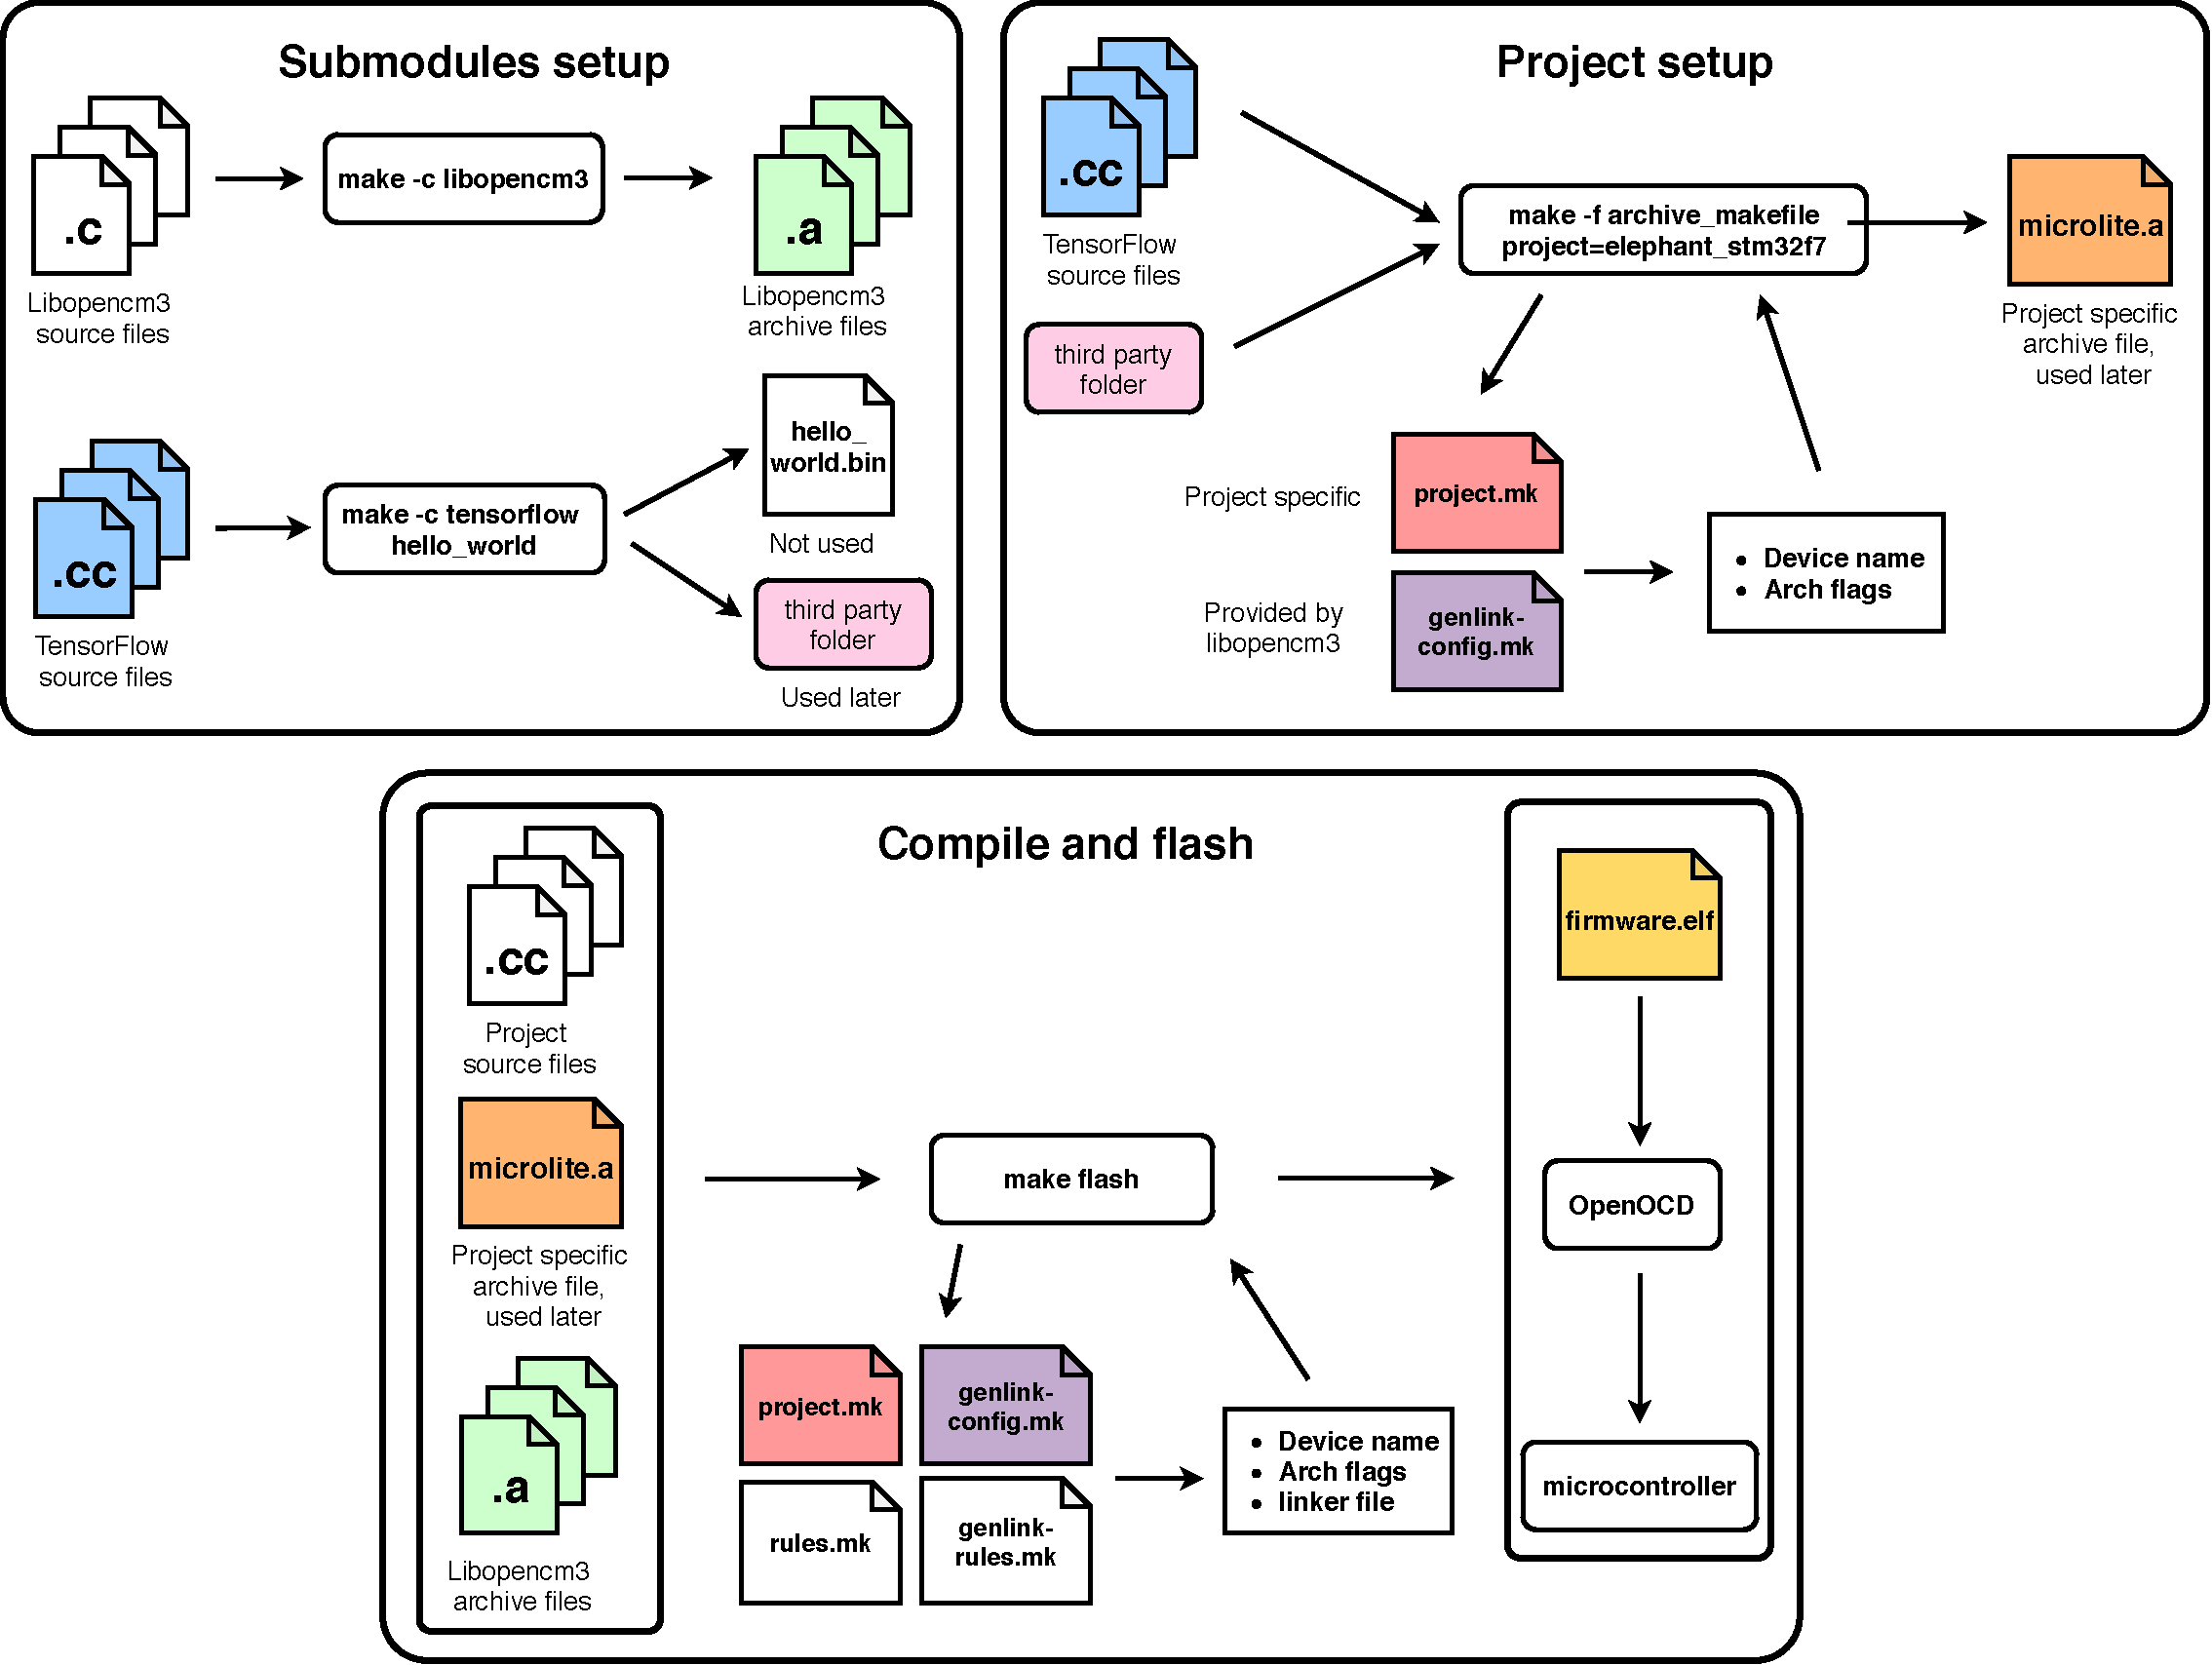
\includegraphics[width=1.0\linewidth]{build_system.pdf} 
        \caption{ Build system of MicroML project.} 
        \label{build_system}
\end{figure}

In \textit{submodules setup} stage we first compile both of the submodules, this step requires two makefiles that are already provided by each submodule.
Compiling libopencm3 creates a group of archive files (static libraries), which contain all platform specific code.
Compiling a TensorFlow Hello World example does not produce any archive files that we would need, however it does execute several scripts which download several different third party files.
TFLite Micro library depends on this files, so does MicroML.
\textit{Submodules setup} stage only has to be executed once.

Whenever we start with a new project that will use ML algorithms, we need to go through \textit{project setup} stage.
From main directory we call make command with \verb|archive_makefile| and define \verb|PROJECT| variable with the name of our project.
\verb|Archive_makefile| looks into \verb|project.mk| and extracts \verb|DEVICE| variable.
Libopencm3's \verb|genlink-config.py| script then with the help of \verb|DEVICE| variable determines which compile flags\footnotemark are needed. 
Afterwards all needed TensorFlow source files and third party files are compiled with this flags and a project specific \verb|microlite.a| archive file is created in our project's folder.

\footnotetext{ For example, flags   \verb|-mcpu=cortex-m7|, \verb|-mthumb|, \verb|-mfloat-abi=hard| and \verb|-mfpu=fpv5-sp-d16| tell gcc compiler that we are compiling for cortex-m7 proccesor, that we want to use thumb instruction set and that we want to use hardware floating point unit with single precision. This flags were generated for STM32F767ZI microcontroller by libopencm3.}

\textit{Compile and flash} stage is then continuously performed during development period.
By calling \verb|make flash| directly in our project folder we compile all project files, \verb|microlite.a| and libopencm3 archive files that were created early.
Libopencm3 helper scripts (\verb|genlink-config.mk| and \verb|genlink-rules.mk|) provide us with microcontroller specific flags and linker script.
After compilation a \verb|firmvare.elf| is created, make then automatically calls OpenOCD, which flashes a microcontroller.

As flashing a big binary to a microcontroller can take a long time, we also created a similar setup for testing inference directly on the host machine.
That way we could test ML specific routines fast and quickly removed any mistakes found on the way.


\subsection{ Running inference on a microcontroller}

TFLite Micro API is fairly simple to use and general enough that it can be copied from project to project without many modifications.
Figure \ref{inference_code} shows a simplified inference code example, copied from our project.
As a first step, we need to define size of \verb|tensor_arena| array, which holds memory input, output, and intermediate arrays.
Exact size of \verb|tensor_arena| is determined by trail and error: we set it to some big value and then decrease it in steps, until the code does not work anymore.

In lines 9 and 10 we an instance of \verb|ErrorReporter| object.
This objects serves as a thin wrapper around platform specific \verb|printf| implementation.
If some part of TensorFlow code crashes, \verb|ErrorReporter| would notify us what went wrong.

In line 13 we pull in our ML model in hex array format that we created with xxd.
\verb|full_quant_model| is defined in a different file, not seen in this example.

In lines 16 to 24 we create an operation resolver.
One way to do it is to specify each needed operation specifically (which is done in the example) or simply pull in all operation implementations.
Latter approach is however not recommended, as it results in a large binary size.
To find out exactly which operations are needed we used online tool Netron\cite{netron}.

In lines 27 and 33 we create an \verb|MicroIinterpreter| instance and allocate memory are to it that we specified with \verb|tensor_arena| earlier.
Lines 37 and 38 assign input and output of the interpreter to new \verb|TfLiteTensor| variables.
This step eases later steps as we can access to input and output more directly.
It also enables us to do two things.
Firstly, variables input and output now actually point to information about specific format of the data: we can found out how many dimensions are needed, what is size of those dimensions and what is expected type of variable (\verb|uint8_t|, \verb|int8_t|, \verb|float|...).
In our test that we ran directly on our laptop we test exactly for these values to confirm that the model will work as expected.
Secondly we now have a way to directly feed data into input, this is done in for loop on line 41.
One of \verb|TfLiteTensor| members is a union variable \verb|data| which contains variables of types.
This type of structure enables us to load input with any kind of data, in our case \verb|int8|.

In line 47 we finally invoke interpreter and run inference on input data.
Whole expression is surrounded with timing functions, which are used to keep track of time spend computing inference.

We finally call \verb|print_results|, which we wrote, where we pass \verb|error_reporter| for printing, \verb|output| for extracting computed probabilities and elapsed time.

After initial setup, we can load data and call invoke as many times we want.

\lstset{style=mystyle}

\begin{figure}[ht] 
    \begin{lstlisting}[language=C++]
// An area of memory to use for input, output, 
// and intermediate arrays.
const int kTensorArenaSize = 200 * 1024;
static uint8_t tensor_arena[kTensorArenaSize];

int main() 
{
    // Debug print setup
    tflite::MicroErrorReporter micro_error_reporter;
    tflite::ErrorReporter *error_reporter = &micro_error_reporter;

    // Map the model into a usable data structure
    const tflite::Model* model = tflite::GetModel(full_quant_tflite);

    // Pull in needed operations
    static tflite::MicroMutableOpResolver<8> micro_op_resolver;
    micro_op_resolver.AddConv2D();
    micro_op_resolver.AddMaxPool2D();
    micro_op_resolver.AddReshape();
    micro_op_resolver.AddFullyConnected();
    micro_op_resolver.AddSoftmax();
    micro_op_resolver.AddDequantize();
    micro_op_resolver.AddMul();
    micro_op_resolver.AddAdd();

    // Build an interpreter to run the model with.
    static tflite::MicroInterpreter interpreter(model, 
                                                micro_op_resolver, 
                                                tensor_arena,
                                                kTensorArenaSize, 
                                                error_reporter);
    // Allocate memory from the tensor_arena
    interpreter->AllocateTensors();

    // Get information about the memory area 
    // to use for the model's input.
    TfLiteTensor* input  = interpreter->input(0);
    TfLiteTensor* output = interpreter->output(0);

    // Load data from image array
    for (int i = 0; i < input->bytes; ++i) {
        input->data.int8[i] = image_array[i];
    }

    // Run the model on this input and time it
    uint32_t start = dwt_read_cycle_counter();
    interpreter->Invoke();
    uint32_t end   = dwt_read_cycle_counter();
    
    // Print probabilites and time elapsed
    print_result(error_reporter, output, dwt_to_ms(end-start));
}
    \end{lstlisting}
    \caption{ Example of TensorFlow Lite inference code in C++.}
    \label{inference_code}
\end{figure}


\subsection{ Wisent board control firmware}
    flow diagram
    cli interface (this should be put somewhere, or not?)

\section{ Server side components and software}

In this section we describe possible server side construction of various frameworks which enable us to receive LoRaWAN message, parse it, store it in a database and present it.
For this thesis we did not implement this specific setup as it was not required for testing purposes, however at IRNAS we use this setup all the time for our IoT products and implementing such system would be trivial.

System that we use consists of different components, each one with a distinct task.
Tools that we use are The Things Network (TTN), Node-RED, InfluxDB and Grafana.
Flow of information and tasks of each tool are presented on Figure \ref{server_side}.

\begin{figure}[ht]
    \centering
    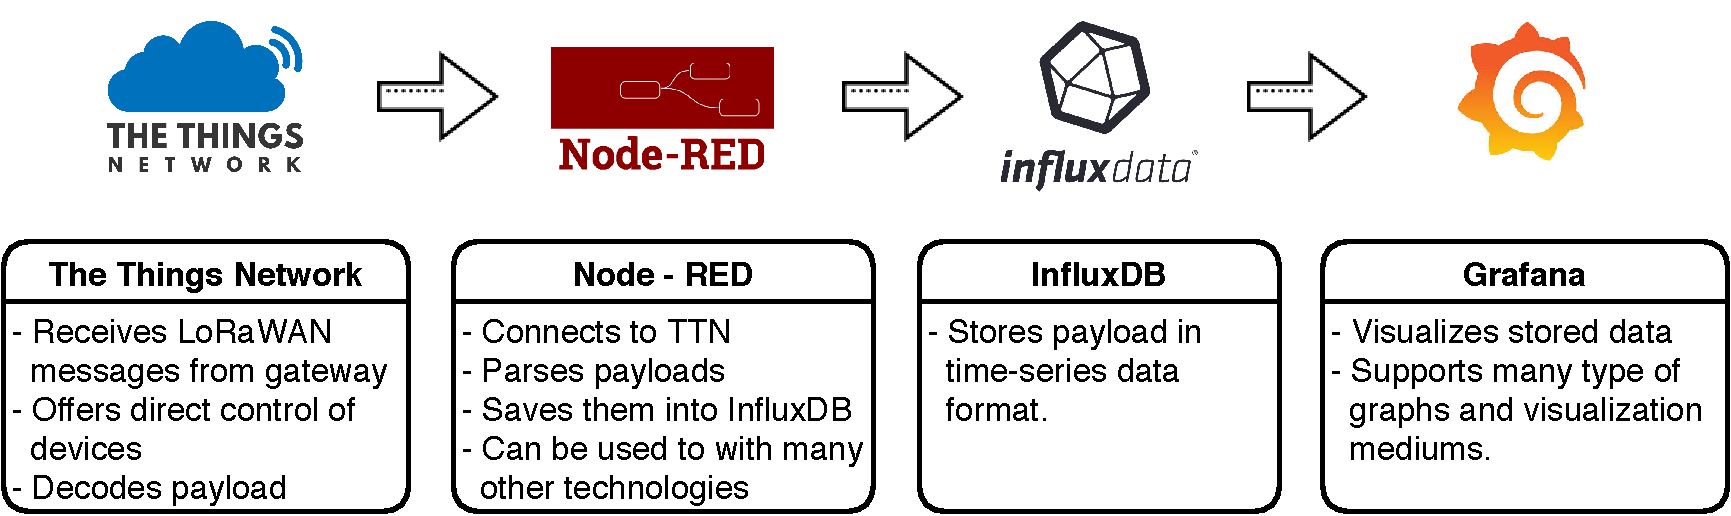
\includegraphics[width=1.0\linewidth]{server_side.pdf} 
    \caption[Server side flow of information.]{Server side flow of information. Icons source:\cite{icons}}
    \label{server_side}
\end{figure}

TTN is responsible for routing packets that are captured by a gateways to the application server.
Since it is open-source and free, anyone can register their gateway device into the network and thus helps to extend it.
TNN is web based, so we can see payload messages directly in the browser.
Since data is usually encoded in binary format, we can provide a decoder script written in JavaScript and TTN will automatically decode each message by it.

Node-RED functions as a glue logic that parses packets and shapes them into format that is required by InfluxDB.
Node-RED provides a browser-based flow editor, where actual programming can be done graphically.
Logic is programmed by choosing different blocks called \textit{nodes} and connecting them together.
This is convenient, as Node-RED provides different nodes for communicating with different technologies, such as MQTT, HTTP requests, emails, Twitter accounts and others.
In our use case we need to use a combination of nodes seen on Figure \ref{nodered_flow}
Node \textit{Elephant Gateway} is connected to a specific application on TTN, which is used for collection of packets from our device in field.
Any packet that will appear in that TTN application will also appear in Node-RED.
Node \textit{Parse packet} extracts information contained in each packet and stores it in a specific format, which is finally send to node \textit{Elephant Database}.

\begin{figure}[ht]
    \centering
    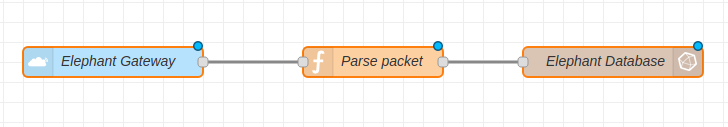
\includegraphics[width=1.0\linewidth]{nodered_flow.png} 
    \caption{ Node-RED flow.}
    \label{nodered_flow}
\end{figure}

\textit{Elephant Database} is connected to InfluxDB, which acts as a time series database.
Any packet that is saved in it is automatically timestamped.

Finally data is visualized in Grafana. 
Grafana is a open source analytics and monitoring solution.
Users define which database is set as source and Grafana provides graphical controls which are at some point converted into SQL like language understandable to InfluxDB.
Grafana provides different types of visualizations, such as graphs, gauges, heat maps, alert lists and others.
In our use case we could display information about various devices in the field, such as battery voltage, number of wakeup triggers, results of each inference and others.

Example of Grafana graph can be seen on Figure \ref{grafana}.

\begin{figure}[ht]
    \centering
    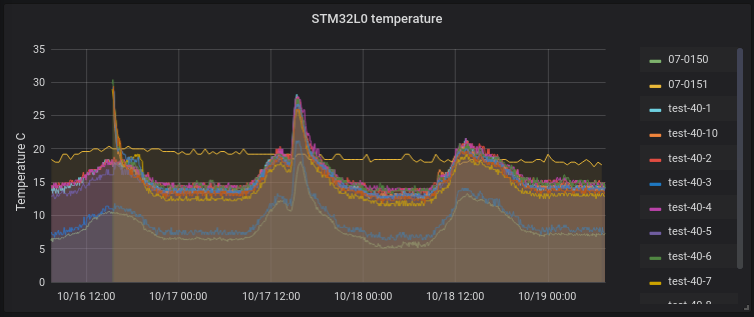
\includegraphics[width=1.0\linewidth]{grafana.png} 
    \caption{ Example of Grafana graph.}
    \label{grafana}
\end{figure}

One important quality of Node-RED, InfluxDB and Grafana is that they can run directly on a embedded Linux system, such as Raspberry Pi, which greatly lowers the cost of hardware that is needed.
